\documentclass[10pt,letterpaper]{book}

\usepackage{outlines}
\usepackage{amsmath}
\usepackage{tikz}
\usepackage{hyperref}
\usepackage{enumitem}
\usepackage{subcaption}
\usepackage{multirow}

\usepackage{float}

\usepackage{slantsc,lmodern}

\usepackage{pgfplotstable,booktabs}
\usepackage{framed}
\definecolor{shadecolor}{rgb}{0.9,0.9,0.9}

\usepackage{gensymb}

\addtolength{\oddsidemargin}{-.875in}
\addtolength{\evensidemargin}{-.875in}
\addtolength{\textwidth}{1.75in}

\addtolength{\topmargin}{-.875in}
\addtolength{\textheight}{1.75in}

\begin{document}


\clearpage
%% temporary titles
% command to provide stretchy vertical space in proportion
\newcommand\nbvspace[1][3]{\vspace*{\stretch{#1}}}
% allow some slack to avoid under/overfull boxes
\newcommand\nbstretchyspace{\spaceskip0.5em plus 0.25em minus 0.25em}
% To improve spacing on titlepages
\newcommand{\nbtitlestretch}{\spaceskip0.6em}
\pagestyle{empty}
\begin{center}
  \bfseries
  \nbvspace[1]
  \Huge
  {\nbtitlestretch\huge
    MECHATRONICS}

  \nbvspace[1]
  \normalsize
  PRINCIPLES, DESIGN, AND ANALYSIS\\
  OF COMPLEX ELECTRO-MECHANICAL SYSTEMS\\
  
  \nbvspace[1]
  \small BY\\
  \Large THADDEUS HUGHES\\[0.5em]

  \nbvspace[2]

  \nbvspace[3]
  \normalsize

  \large
  PUBLISHED IN THE WILD
  \nbvspace[1]
\end{center}


\tableofcontents

\chapter{Introduction}
 {\slshape \scshape ``Insert a Witty Quote Here" - And That Kid, was Albert Einstein}

Mechatronics is an amalgam of mechanical electronics - systems that contain both mechanical and electrical components.

\chapter{Construction}
 {\slshape \scshape ``The first little pig was very lazy. He didn't want to work at all and he built his house out of straw. The second little pig worked a little bit harder but he was somewhat lazy too and he built his house out of sticks. The third little pig worked hard all day and built his house with bricks. It looked like it could withstand the strongest winds." - English Folk Tale}
 
 The parable of the three little pigs reminds us that how we build things is important. And while at first blush, the story seems to be about how you should always build strong out of brick, sometimes we should learn from the first pig, and build fast. Having a suite of different fabrication techniques at hand can be incredibly handy.
 
 \section{Materials}
 
 Before we discuss how to make something and put it together, let's have a brief aside to what different things we can make things out of. There are a lot of different materials, all with different properties. Some important ones are:
 
 \begin{itemize}
 	\item Density (Weight)
 	\item Stiffness
 	\item Hardness
 	\item Strength
 	\item Toughness
 	\item Thermal Capabilities
 	\item Frictional and Chemical Interactions
 \end{itemize}
 
 You'll notice that stiffness, strength, hardness, and toughness are all different characteristics- although in common parlance, we might use them as synonyms. They are, however, distinctly different properties in engineering.
 
 To show this, we'll first consider a "stress-strain curve". This curve is created by pulling on a specimen of material like shown, interpreting the force and deflection data into "stress" $\sigma$ (force per cross-sectional area) and "strain" $\epsilon$ (percent deflection).
 
 \begin{figure}[H] \centering
 	\begin{tikzpicture}[x=1.0in, y=1.0in]
 		\draw[ ] (-0.1,0) -- (0.1,0) -- (0.1, 1) -- (-0.1, 1) -- cycle;
 		\draw[->] (0,-0.1)--(0,-0.5) node[pos=0.5, right]{$F$};
 		\draw[->] (0,1.1)--(0,1.5) node[pos=0.5, right]{$F$};
 	\end{tikzpicture}
 	\qquad
 	\begin{tikzpicture}[x=1.0in, y=1.0in]
 		\draw[->] (0,0)--(3,0) node[pos=0.5, below]{$\epsilon$};
 		\draw[->] (0,0)--(0,2) node[pos=0.5, left]{$\sigma$};
 		\draw[blue, thick] (0,0)--(1,1);
  		\draw[gray] (1,1)--(1.8,1.8);
 		\draw[red, thick]  (1,1) .. controls (1.5,1.5) and (2.0,1.5) .. (2.5,1.25);
 		\draw[purple, ->] (2,1.4)--(0.6,0);
 	\end{tikzpicture}
 \end{figure}
 
 The portion of the curve that is linear (highlighted in blue) is referred to as the 'elastic' portion. When the material is operating in this region, it will always snap back (think of a spring). If, however, we dip into the red portion of the curve (called the 'plastic' portion), when we release the material, it will have permanently deformed (following the purple arrow).
 
 The key aspects of the curve can be boiled down into a few properties.
 
 \begin{itemize}
 	\item $E$ - Young's Modulus, or the Elastic Modulus, is the slope of the elastic portion of the curve. A higher $E$ denotes a stiffer material.
 	\item $\sigma_{y}$ - Yield Strength, is the highest stress seen in the elastic portion of the curve.
 	\item $\sigma_{UTS}$ - Ultimate Tensile Strength, is the highest stress the material can see.
 	\item Percent Elongation at Break - the highest strain seen by the material before it breaks. A higher elongation means the material is more 'ductile', while a smaller one means the material is more 'brittle'.
 	\item Modulus of Toughness - The area under the curve, which represents how much energy the material can absorb (think about a shock absorber- it deforms a lot while resisting the load, so can absorb a lot of energy). Usually materials that are very brittle have low toughness.
 \end{itemize}
 
 Some good places to obtain material properties are:
 
 \begin{itemize}
 	\item \href{http://www.matweb.com/search/DataSheet.aspx?MatGUID=3a2e111b27ef4e5d813bad6044b3f318&ckck=1}{\color{red}MatWeb} has a wide range of material properties.
 	\item \href{https://www.makeitfrom.com/}{\color{red}MakeItFrom} has a similarly wide range of materials, and includes a comparison tool to help evaluate different options.
 \end{itemize}
 
 Hardness is not measured by this graph, and is a more subjective property. There are many different scales. You may have heard of the Mohs scale, introduced to determine the hardness of different rocks based on which can scratch each other. Scratching is generally generally the reason we care about hardness, so such subjective scales are fine. However, most engineering measures will work by indenting an object and measuring how much of an indentation was left behind. There are many different scales that are better suited to different materials.
 
 Brinell and Rockwell scales (there are different flavors of these) are well suited to metals.
 
 "Shore" or "Durometer" scales are suited to measuring elastomers (i.e. rubber). Again it is important to make sure the scales are the same - "90A" is much softer than "90D" durometer! Elastomers are much harder to measure in other ways, and are often specced only by their durometer. While this is technically only a measure of hardness, it correlates reasonably well to other material properties like overall stiffness (harder being stiffer) and grip (softer being more interactive, or frictional).
 
 The thermal properties of a material are important. There are three main ones to keep in mind if you are dealing with heat:
 \begin{itemize}
 	\item Thermal Conductivity - a measure of how well the material transfers heat. If you're designing a heat sink, you want a high thermal conductivity.
 	\item Melting Point or Glass Transition Temperature - you obviously need to make sure your part doesn't outright melt, but you should also have a bit of margin, as the phenomenon called 'creep' can cause parts that are at elevated temperatures to shift and bend over time, even though below melting point.
 	\item Coefficient of Thermal Expansion - As things heat up, they expand! If you're working with tight-tolerance equipment (or extreme temperatures), you may need to keep an eye on this.
 \end{itemize}
  
 Frictional characteristics and chemical interactions are very complex, and if you care about these, will require some research beyond mere datasheets.
 
 \section{Form Factors}
 
 Just because the material you want exists, doesn't mean it's widely available in the shape you want. There are a lot of different shapes you can get things in.
 
 \subsection{Cast from Ingnot}
 
 Casting refers to pouring molten material into a mold to produce a complex shape. This shape isn't perfect, as the mold is usually made of sand (in order to withstand the molten metal) and the pouring process can introduce voids and imperfections, so the material properties are usually not as good. Cast parts have notably inferior material properties from billet or 'forged' counterparts.
 
 \subsection{Billet and Plate}
 "Billet" material has been poured in a more tightly controlled environment. The resulting material is free of voids and has superior mechanical properties. You can obtain billet plate, bars, or round stock of nearly any material. This material can be held to reasonable tolerances (and by its simple-shaped nature, can be brought into exact dimension by machining quite easily).
 
 \subsection{Extrusions}
 "Extruded" material is material that has been squeezed through a die- think of a pasta machine. This die can be anywhere from a simple shape like a flat bar, to box tubing, to a very complicated profile with t-slots such as 80/20. Aluminum is the most common material to be extruded. Extrusions have good material properties, and can be held to tight tolerances.
 
  \begin{figure}[H]
	\centering
	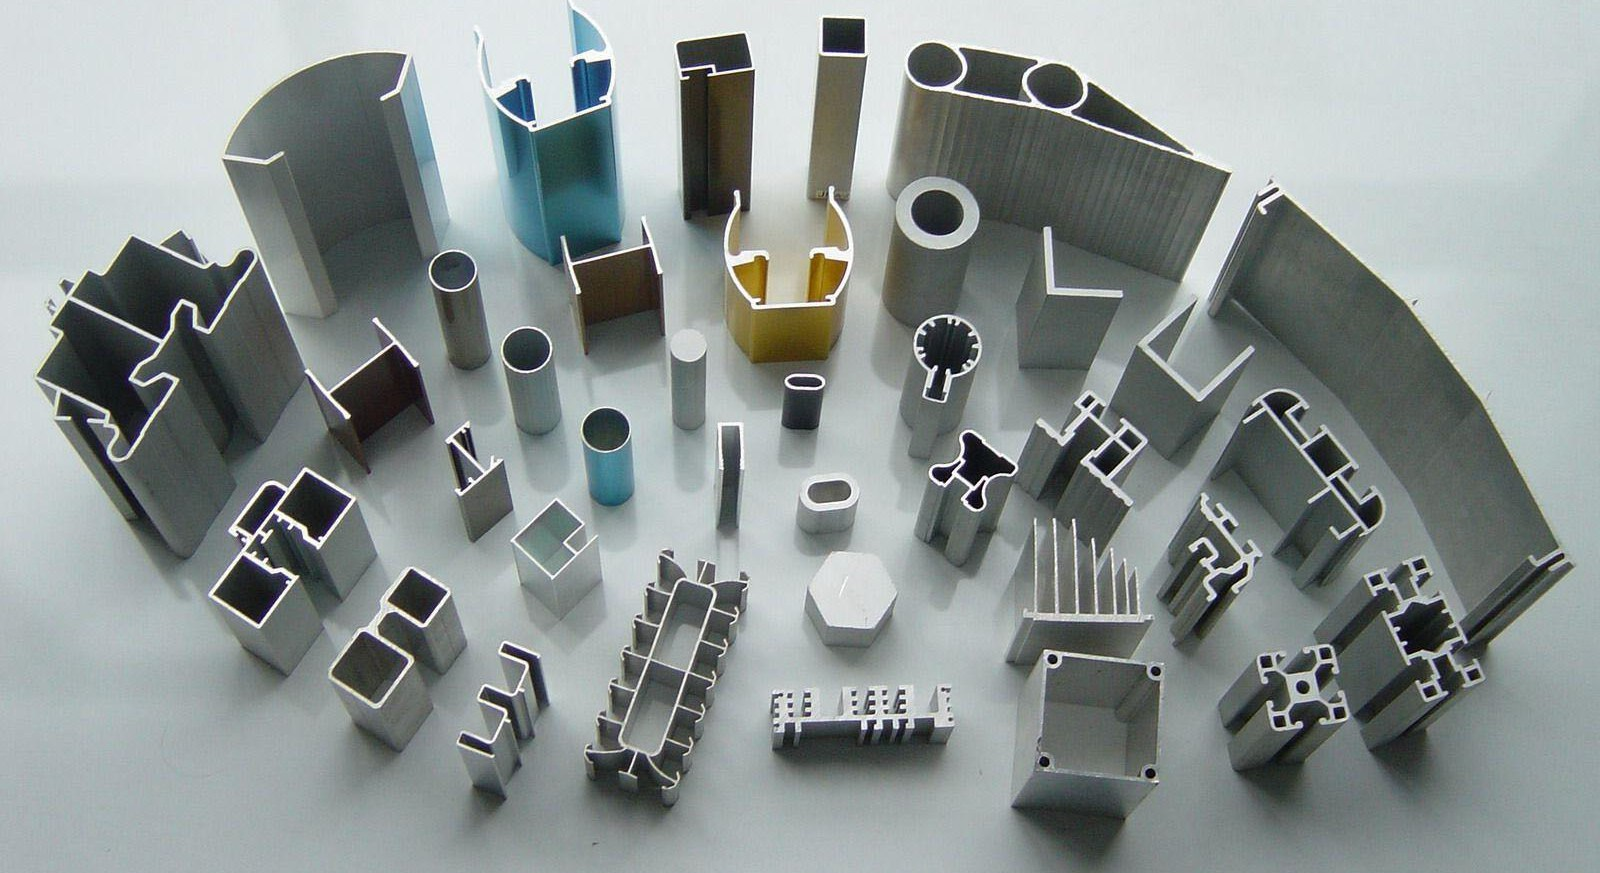
\includegraphics[width=0.8\textwidth]{imgs/extrusions.jpeg}
	
	\caption{Various Extrusions}
\end{figure}
 
 \subsection{Welded / DOM tubing}
 Steel tubes are usually formed by taking sheet and rolling it into a tube, and then welding it together. This process leaves a weld seam which can produce odd material properties, produce dimensional issues (as when making telescoping tubes), or make manufacturing annoying (as the weld is difficult to drill through). 
 
   \begin{figure}[H]
	\centering
	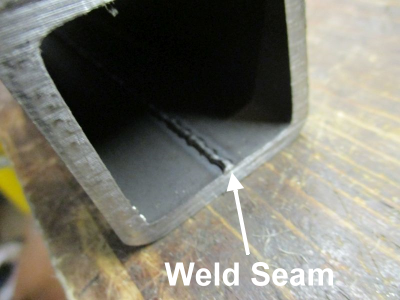
\includegraphics[width=0.4\textwidth]{imgs/welded_tube_seam.png}
	
	\caption{Weld Seam on Tubing}
\end{figure}
 
 DOM (Drawn-over-mandrel) or Seamless tubing further processes this tubing to remove the inner seam and produce a product as if it were extruded.
 
 \subsection{Sheet}
 Material that is sold as 'sheet' rather than 'plate' usually has little-to-no straightness tolerance (in especially thin gagues, it might even be sold as rolls).
 
 \section{Manufacturing Processes}
 
 Once you have a material you like in a shape you can use, you (probably) have to cut or form it into the final shape you want. There are nearly infinite ways of doing this, but here are the most common.
 
 \subsection{Casting/Sintering/Forging}
 
 Casting, sintering, and forging are manufacturing methods which generally require a lot of tooling in order to accomplish, so are generally not suitable for quick-turnaround prototypes such as we need. Some notes, though:
 
 \begin{itemize}
 	\item Casting can produce very complex shapes (like engine blocks), but the material (as mentioned before) may end up with lots of voids.
 	\item Forging (essentially blacksmithing on an industrialized scale) can produce fairly complex shapes (like crankshafts), while preserving (and even enhancing) material properties.
 	\item Sintering is compressing and heating powder in a mold. This can produce somewhat simple parts with good material properties and no draft- many small gears are made this way.
 \end{itemize}
 
 \subsection{Machining}
 
 Machining is a broad term, but generally refers to cutting material away with a sharp tool. There are many tools that fall into this category, but there are three that are the most essential:
 
 \begin{figure}[H]
	\centering
	\begin{subfigure}[b]{.24\linewidth}
		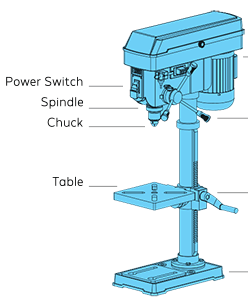
\includegraphics[width=0.95\textwidth]{imgs/drillpress.png}
		\caption{Drill Press}
	\end{subfigure}	\begin{subfigure}[b]{.34\linewidth}
		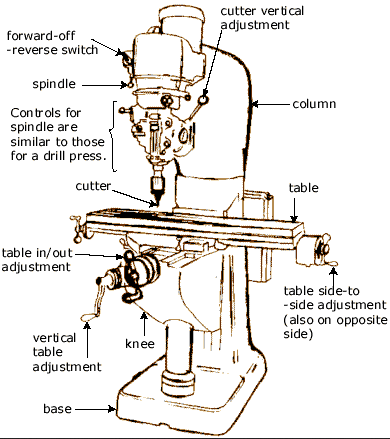
\includegraphics[width=0.95\textwidth]{imgs/mill.png}
		\caption{Milling Machine}
	\end{subfigure}	\begin{subfigure}[b]{.4\linewidth}
		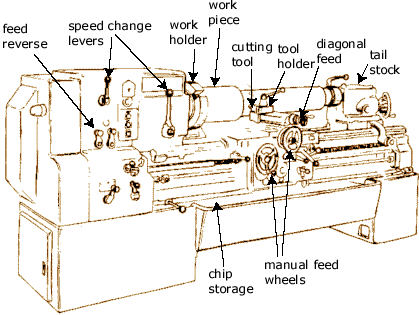
\includegraphics[width=0.95\textwidth]{imgs/lathe.png}
		\caption{Lathe}
	\end{subfigure}	
	
	\caption{The Most Common Machining Tools}
\end{figure}

 \begin{enumerate}[label=\alph*]
 	\item Drill Press - this has a rotating spindle, where drillbits can be inserted, and a fixed table, where the work is clamped.
 	\item Milling Machine - A tool with a rotating spindle, where drillbits and mill bits (end mills) can be inserted, and a table that moves in X, Y, and Z with respect to the spindle.
 	\item Lathe - A tool with a rotating spindle, where the workpiece is held, and a carriage which holds cutting tools that shape the exterior of the work. Additionally, a tailstock can accept drill bits.
 \end{enumerate}
 
 \begin{figure}[H]
	\centering
	\begin{subfigure}[b]{.19\linewidth}
		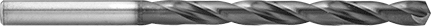
\includegraphics[width=0.95\textwidth]{imgs/drillbit.png}
		\caption{Drill Bit}
	\end{subfigure} \begin{subfigure}[b]{.19\linewidth}
		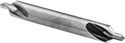
\includegraphics[width=0.95\textwidth]{imgs/centerdrill.png}
		\caption{Centerdrill}
	\end{subfigure}	\begin{subfigure}[b]{.19\linewidth}
		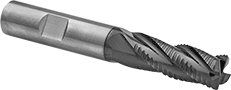
\includegraphics[width=0.95\textwidth]{imgs/endmill.png}
		\caption{End Mill}
	\end{subfigure}	\begin{subfigure}[b]{.19\linewidth}
		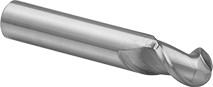
\includegraphics[width=0.95\textwidth]{imgs/ball_endmill.png}
		\caption{Ball End Mill}
	\end{subfigure}\begin{subfigure}[b]{.19\linewidth}
		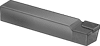
\includegraphics[width=0.95\textwidth]{imgs/lathetool.png}
		\caption{Lathe Tooling}
	\end{subfigure}	
	
	\caption{Machine Tooling}
\end{figure}

 \begin{enumerate}[label=\alph*]
 	\item Drillbits drill holes. The spiral flutes on the outside may be sharp, but they generally aren't sharp or hard enough to actually cut metal. They work with jacobs chucks, which are designed to only transmit vertical force and torque.
 	\item Centerdrills are used to start holes. They are short and stubby, so don't deflect much.
 	\item End Mills cut on all surfaces- they are all ground to be sharp and cut. This means they can cut on the side, and produce side loads- so they should not be put in jacobs chucks in drill presses!
 	\item Ball End Mills are an example of a more sophisticated end mill. There are many different shapes. This one enables smooth contours to be made.
 \end{enumerate}
 
 
 There are lots of variations on these machines- combinations of these exist, and 4- and 5- axis mills (where the head or table tilt on the fly) also exist.
  
 Turning is the process of spinning the work and using a fixed cutter to shape it.
 
\begin{figure}[H]
	\centering
	\begin{subfigure}[b]{.24\linewidth}
		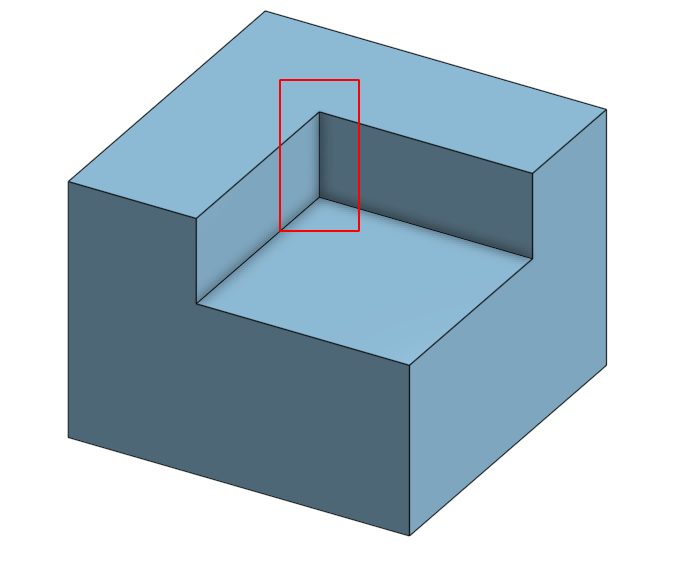
\includegraphics[width=0.9\textwidth]{imgs/nonmill_sharpins.png}
		\caption{Sharp Inside Corner}
	\end{subfigure}	\begin{subfigure}[b]{.24\linewidth}
		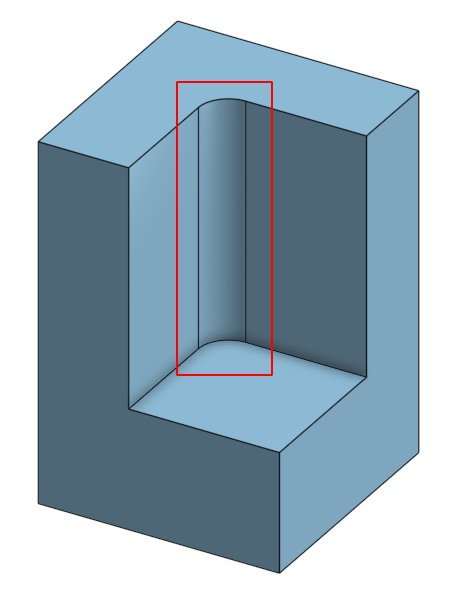
\includegraphics[width=0.9\textwidth]{imgs/nonmill_dtod.png}
		\caption{Too Deep Radius}
	\end{subfigure}	
	
	\caption{Geometries Problematic for Machining}
\end{figure}

 \begin{enumerate}[label=\alph*]
 	\item Sharp Inside Corner - This cannot be made, as it would require an infinitely small diameter tool.
 	\item Too Deep Radius - This radius is 0.25", and it is 2" tall; this is a ratio of depth-to-diameter of 4:1, which is a suboptimal ratio. Ideally, this ratio would be no more than 3:1.
 \end{enumerate}
 
 \subsection{Broaching}
 
 But how do we make splines, keyways, and hexes in things? Those need infinitely sharp corners! Great question! We broach them. This is done by first drilling a hole of the appropriate diameter, and then inserting a broaching tool into the hole. The tool is then pushed through with a press. Each tooth of the broach takes off gradually more material until the final shape is achieved.
 
 \begin{figure}[H] \centering
 	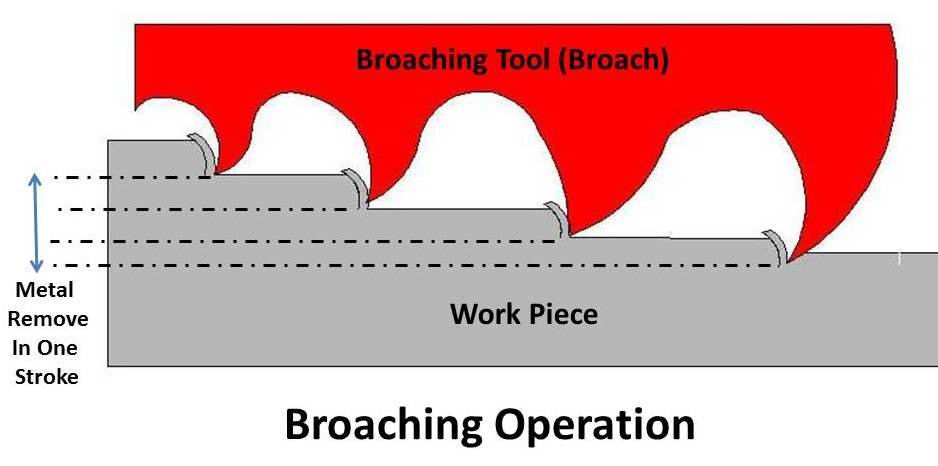
\includegraphics[width=\textwidth]{imgs/broach_detail.jpeg}
 	\caption{Broach Detail}
 \end{figure}
 
 \begin{figure}[H] \centering
 	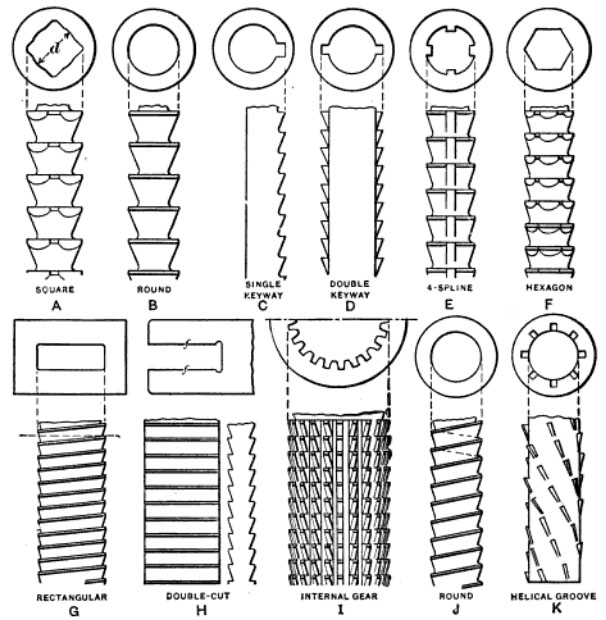
\includegraphics[width=0.7\textwidth]{imgs/broach_examples.jpeg}
 	\caption{Broach Examples}
 \end{figure}
 
 \subsection{Path Cutting}
 
 Path cutting is a term I made up that encompasses any sort of 2-dimensional X/Y cutting with a thin beam.
 
 \begin{figure}[H]
		\centering
		\begin{subfigure}[b]{.24\linewidth}
			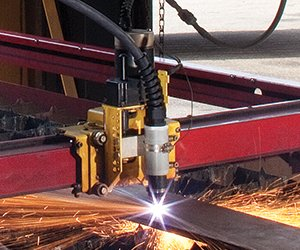
\includegraphics[width=0.9\textwidth]{imgs/plasmacut.jpeg}
			\caption{Plasma Cutting}
		\end{subfigure}\begin{subfigure}[b]{.24\linewidth}
			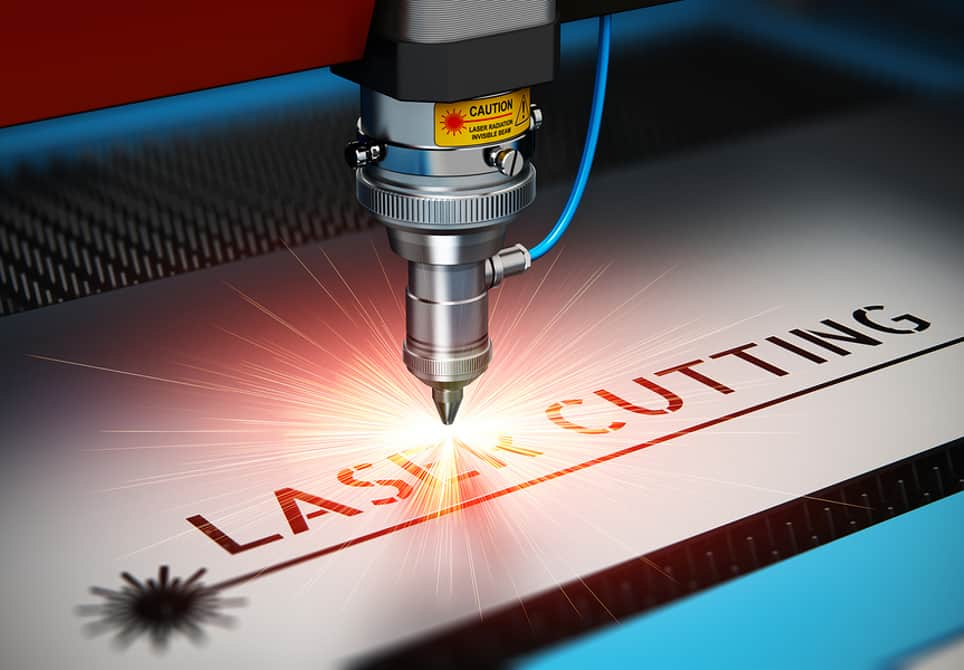
\includegraphics[width=0.9\textwidth]{imgs/lasercut.jpeg}
			\caption{Laser Cutting}
		\end{subfigure}\begin{subfigure}[b]{.24\linewidth}
			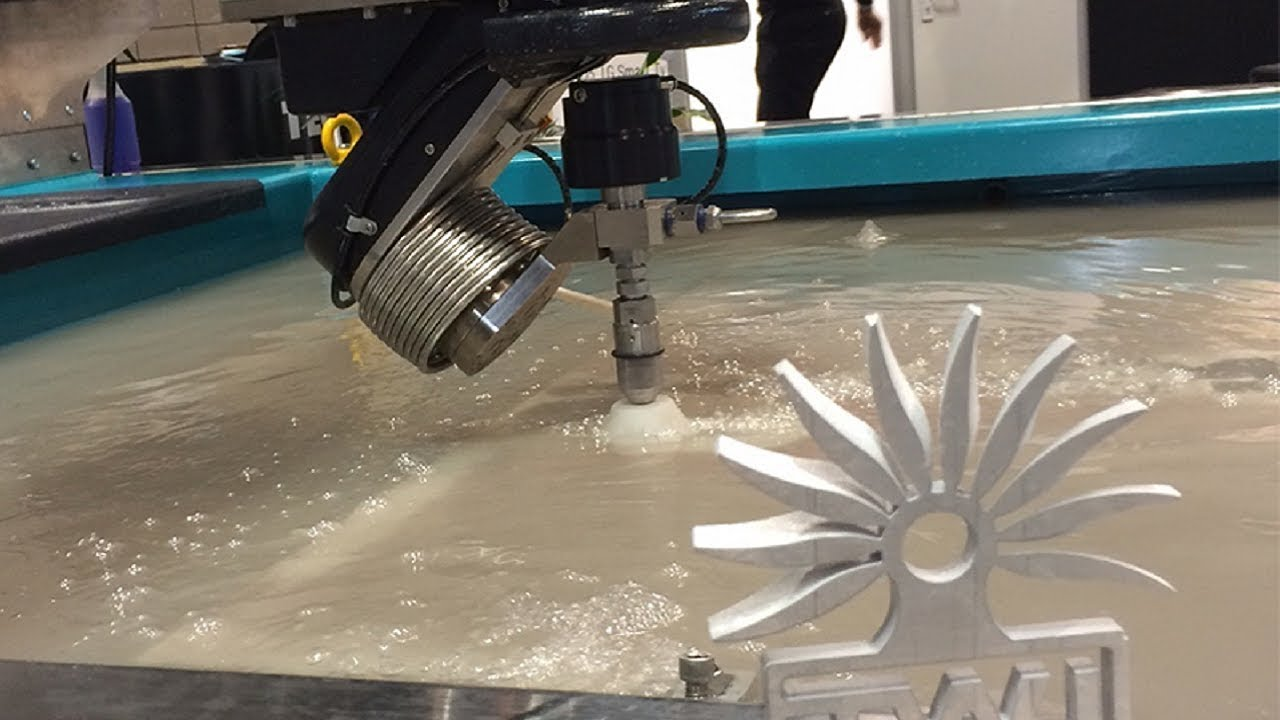
\includegraphics[width=0.9\textwidth]{imgs/waterjet.jpeg}
			\caption{Waterjet Cutting}
		\end{subfigure}\begin{subfigure}[b]{.24\linewidth}
			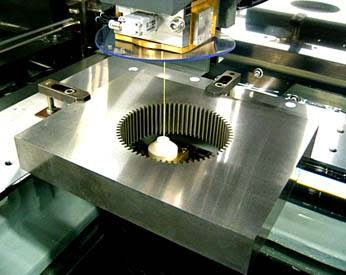
\includegraphics[width=0.9\textwidth]{imgs/edm.jpeg}
			\caption{EDM Cutting}
		\end{subfigure}
	\end{figure}
 
 \begin{enumerate}[label=\alph*]
  	\item Plasma cutting: melting metal and using pressurized air to blow it away. The tolerances are usually good for large shapes, but not for precision work.
 	\item Laser cutting: melting material with a laser and either vaporizing it or using pressurized air to blow it away. Hobby lasers can cut some plastics and plywood, while industrial systems can cut metal. The tolerances are usually acceptable with these machines ($\pm 0.020"$)
 	\item Waterjet cutting: High-pressure water is mixed with garnet sand and blasted at material, rapidly abrading it. The tolerances are usually good with this process ($\pm 0.010"$)
 	\item EDM (electro-discharge-machining): A wire is fed through material and electrified. The electrification 'zaps' away material next to the wire. The tolerances with this process can be impeccable ($\pm 0.001"$ or better) 
\end{enumerate}
 	
 	These all allow us to overcome the depth-to-diamter ratio imposed by milling, and can often be much quicker setup than traditional machining, though they all come with their own drawbacks.
 
 The first limitation is the width of the beam. Since a finite-ly sized beam muse be used, infinitely sharp interior corners cannot be made.
 
 \begin{figure}[H] \centering
 	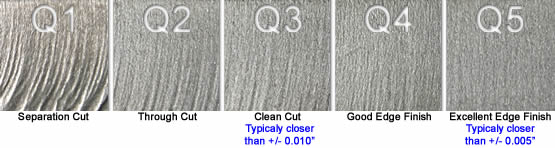
\includegraphics[width=0.9\textwidth]{imgs/waterjet_draft.jpeg}
 	\caption{Waterjet Draft and Surface Quality}
 \end{figure}
 
 \begin{figure}[H] \centering
 	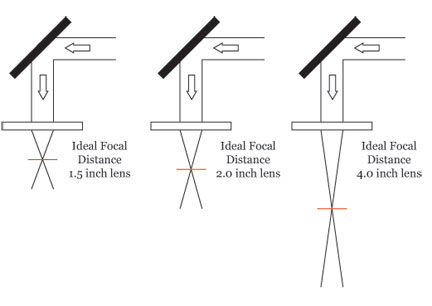
\includegraphics[width=0.5\textwidth]{imgs/lasercut_focus.jpeg}
 	\caption{Laser Cutter Focus}
 \end{figure}
 
 The next consideration that must be made is draft. Laser-cutters typically have a point in the thickness where the beam is focused to. This means that the laser doesn't cut a line in its cross-section, but rather an X. Thus the resulting shape is two-dimensional. With a waterjet or plasma cutter, the draft grows exponentially. This may be acceptable, or require further post-machining to bring it into specification.
 
 Draft (and power) also limits how thick of material can feasibly be cut with these processes. EDM is the exception though- it can cut extremely thick material.
 
 \subsection{Sheet Forming}
 
 Sheet forming is a versatile process of making parts from, well, sheet. Sheet may be cut either with a stamping operation, or with a path-cutting operation to form a blank. This blank can then be loaded in and undergo one of several processes.
 
 	\begin{figure}[H]
		\centering
		\begin{subfigure}[b]{.24\linewidth}
			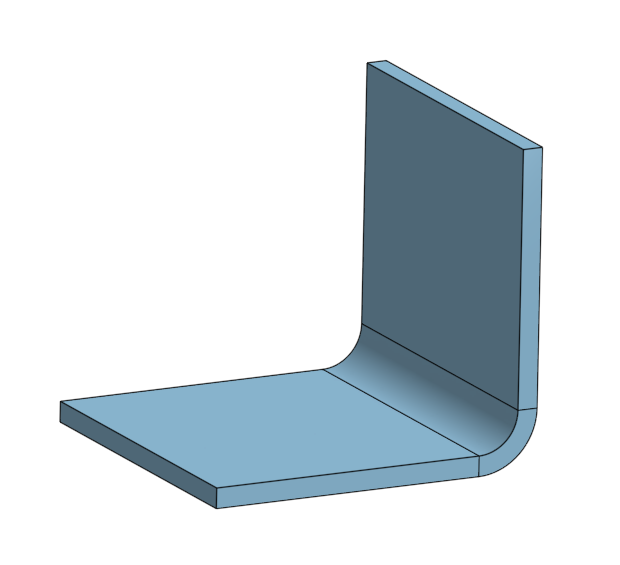
\includegraphics[width=0.9\textwidth]{imgs/sheet_bend.png}
			\caption{Bend}
		\end{subfigure}\begin{subfigure}[b]{.24\linewidth}
			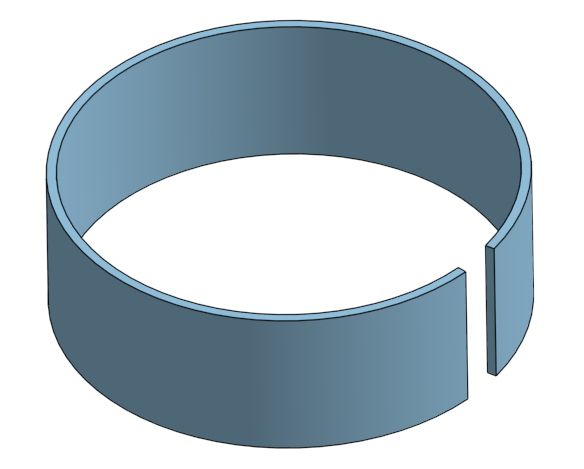
\includegraphics[width=0.9\textwidth]{imgs/sheet_roll.png}
			\caption{Rolling}
		\end{subfigure}\begin{subfigure}[b]{.24\linewidth}
			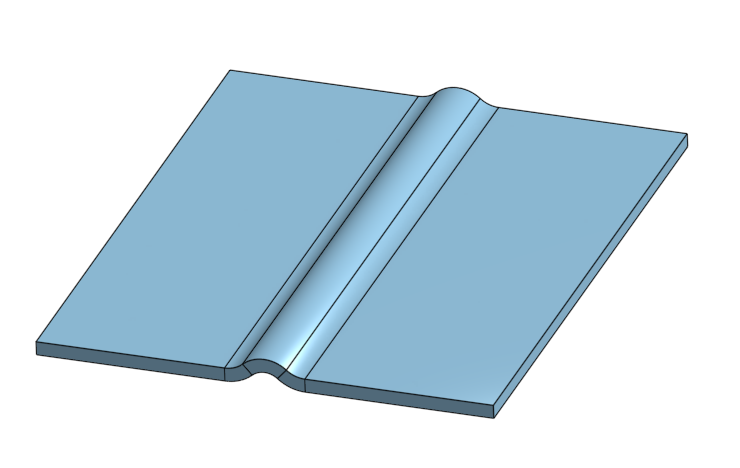
\includegraphics[width=0.9\textwidth]{imgs/sheet_beadroll.png}
			\caption{Bead Rolling}
		\end{subfigure}\begin{subfigure}[b]{.24\linewidth}
			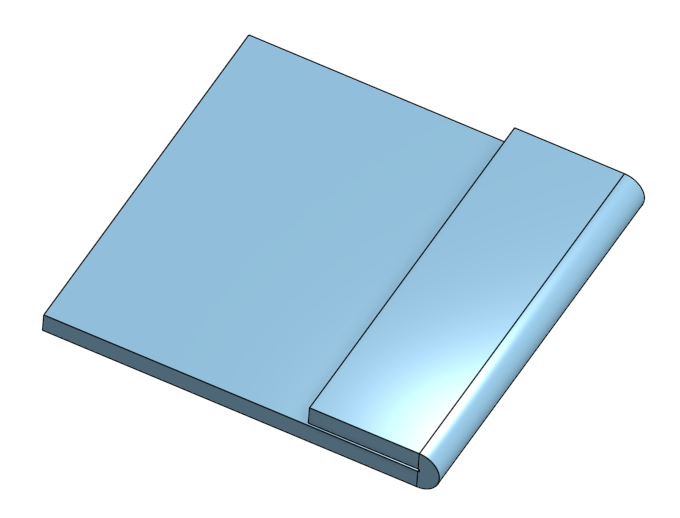
\includegraphics[width=0.9\textwidth]{imgs/sheet_hem.png}
			\caption{Hemming}
		\end{subfigure}
		\caption{Rudimentary Sheetmetal Operations}
	\end{figure} 
 
 \begin{enumerate}[label=\alph*]
 	\item Bending - a simple bend is made on a linear portion of the flat pattern. This can be done with a finger bender, press brake, or (in a pinch) a vise with a hammer.
 	\item Rolling - a portion of the blank is rolled into an arc.
 	\item Bead rolling - a bead is rolled along a flat portion of the part. This provides some additional stiffness.	
 	\item Hemming - a bend is made, but bent all the way to 180 degrees in order to provide a smooth, radiused outer corner (and some additional stiffness). This can be done with a finger bender or press brake, and additional clamping to finish the hem.
 	\end{enumerate}
 	
 	Most CAD packages have tools to design parts made with sheetmetal. You can draw up the bent part, and then the CAD package will determine how to 'unfold' and produce a flat pattern that can be cut out.
 	
 	These operations are typically done with metal, but nothing prevents you from doing it with plastic. Polycarbonate can be bent like sheetmetal. Polypropylene, polycarbonate, acrylic, PETG amongst others can also be heated (i.e. with a heat gun) and then bent by hand.
 	
 	\subsection{Welding and Brazing}
 	
 	Welding and brazing are very important manufacturing methods. They enable large, complex structures to be made from smaller simple ones, without fasteners that might fail. However, it can be quite time consuming, requires time consuming labor, and creates non-servicable structures.
 	
 	\begin{figure}[H]
		\centering
		\begin{subfigure}[b]{.24\linewidth}
			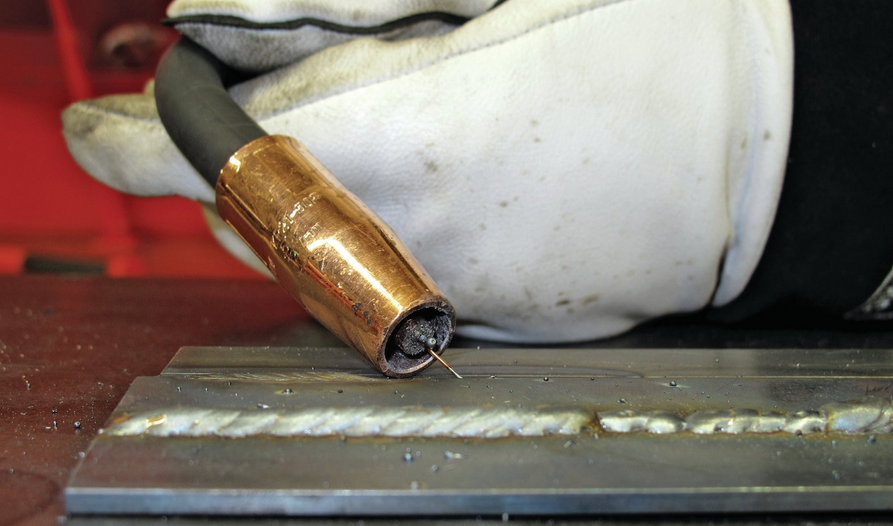
\includegraphics[width=0.9\textwidth]{imgs/mig.png}
			\caption{MIG Welding}
		\end{subfigure}\begin{subfigure}[b]{.24\linewidth}
			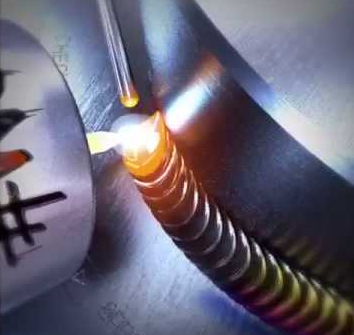
\includegraphics[width=0.9\textwidth]{imgs/tig.png}
			\caption{TIG Welding}
		\end{subfigure}\begin{subfigure}[b]{.24\linewidth}
			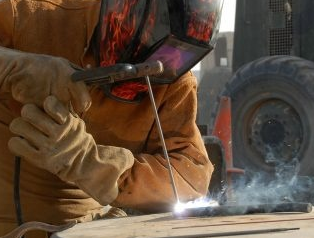
\includegraphics[width=0.9\textwidth]{imgs/arcweld.png}
			\caption{Stick Welding}
		\end{subfigure}\begin{subfigure}[b]{.24\linewidth}
			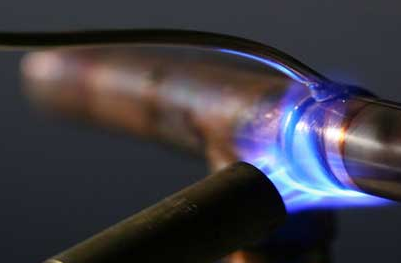
\includegraphics[width=0.9\textwidth]{imgs/braze.png}
			\caption{Brazing}
		\end{subfigure}
		\caption{Quick Pins}
	\end{figure}
 	
 	\begin{enumerate}[label=\alph*]
 		\item MIG (Metal-Inert-Gas) welding: an electric arc is created between filler wire and the workpiece, which melts both the wire and the workpiece. The arc is shielded by inert (or semi-active) gas to control chemical reactions. The wire is advanced at a constant rate into the workpiece. This is the easiest method to learn, but provides the least amount of control, and has the lowest capacity for superior results.
 		
 		\item TIG (Tungsten-Inert-Gas) welding: an electric arc is created between a fixed tungsten rod and the workpiece, melting the work but not the tungsten. The arc is shielded by inert gas to eliminate chemical reactions. Filler rod is advanced manually and separately into the molten work. This method is much harder to learn, but provides the most amount of control, with the highest capacity for superior results.
 		
 		\item Stick (or Arc) welding: an electric arc is created between a rod containing flux and filler metal and the workpiece, melting both the rod and the workpiece.. The arc is shielded by the vaporizing flux. This method is hard to learn, but provides good control, and works best outdoors, so is quite common in the construction and pipeline industries.
 		
 		\item Brazing: heat is generated (either by a TIG torch, or a flame torch) and directed at the work, but not hot enough to melt the work. Brazing material, which will melt at this surface temperature, is fed onto the work, melting and flowing across it. As it solidifies, it adheres to the base metal.
 		
 	\end{enumerate}
 		
	\section{Fasteners}
	So you've made some parts, now it's time to put them together. How are you going to do it? CAD Constraints won't help you now! You need real fasteners!
	
	\subsection{Pins}
	The simplest fastener is a pin. Pins prevent holes in plates from shearing past each other, by putting all of the load through the pin. There are a couple different flavors that let you do different things.
	
	Quick pins allow users to easily make adjustments or reconfigurations to equipment. They are easily insertable/removable, usually without any special tools.
	
	\begin{figure}[H]
		\centering
		\begin{subfigure}[b]{.32\linewidth}
			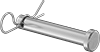
\includegraphics[width=0.7\textwidth]{imgs/cpin.png}
			\caption{Clevis Pin}
		\end{subfigure}\begin{subfigure}[b]{.32\linewidth}
			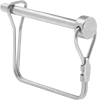
\includegraphics[width=0.7\textwidth]{imgs/wlpin.png}
			\caption{Wire-Locking Pin}
		\end{subfigure}\begin{subfigure}[b]{.32\linewidth}
			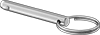
\includegraphics[width=0.7\textwidth]{imgs/bdpin.png}
			\caption{Ball-Detent Pin}
		\end{subfigure}
		\caption{Quick Pins}
	\end{figure}
	
	\begin{enumerate}[label=\alph*]
		\item Clevis pins - these are loose tolerance pins which have a hole for a locking (R-shaped) pin or wire to go through.
		\item Wire-Locking pins - these serve the same purpose as clevis pins, but use a spring-loaded wire to keep the pin captive.
		\item Ball-Detent pins - these serve the same purpose as clevis pins, but use a spring-loaded ball detent to keep the pin captive. These can be pulled/pushed in without and additional steps.
	\end{enumerate}
	
	
	Precision pins serve a nearly opposite purpose- they are permanent instalations, but provide extremely tight tolerances when used right. They allow for installation/detachment of components with high repeatability in locational positioning. It's not uncommon to see precision equipment register together with pins, and then be bolted together in addition to the pins. Pins also can provide higher load transferral since they do not have the stress concentrators that bolts do.
	
	\begin{figure}[H]
		\centering
		\begin{subfigure}[b]{.24\linewidth}
			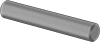
\includegraphics[width=0.7\textwidth]{imgs/dpin.png}
			\caption{Dowel Pin}
		\end{subfigure}\begin{subfigure}[b]{.24\linewidth}
			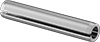
\includegraphics[width=0.7\textwidth]{imgs/spin.png}
			\caption{Spring Pin}
		\end{subfigure}\begin{subfigure}[b]{.24\linewidth}
			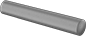
\includegraphics[width=0.7\textwidth]{imgs/tpin.png}
			\caption{Taper Pin}
		\end{subfigure}\begin{subfigure}[b]{.24\linewidth}
			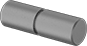
\includegraphics[width=0.7\textwidth]{imgs/shpin.png}
			\caption{Shear Pin}
		\end{subfigure}
		\caption{Precision Pins}
	\end{figure}
	
	\begin{enumerate}[label=\alph*]
		\item Dowel pins - these are tight-tolerance pins that can be pressed into one part's hole, and have a loose fit on the other.
		\item Spring pins - these are pins formed from coiled metal, intended to be pressed in like a dowel pin, but have some give to them so can be used with looser-tolerance holes.
		\item Taper/scotch pins - these are like dowel pins, but they are slightly tapered, so they wedge into multiple parts like a nail.
		\item Shear pins - these are pins specifically designed to fail at a specified load, which prevents damage to equipment down-the-line.
	\end{enumerate}
	
	\subsection{Threads}
	
	Threaded fasteners (bolts, nuts, and screws) are a ubiquitous solution. There's an age old question of what is a 'screw' versus a 'bolt' and the answer is merely in application- if it goes into a nut, it's a bolt. Otherwise, it's a screw. So, anything said about screws is true of bolts and vise-versa. Threaded fasteners are denoted by:
	
	\begin{itemize}
		\item The major diameter of the thread.
		\item The thread pitch, or threads-per-inch. Metric bolts are specced by the pitch (a M5x0.8 has 0.8mm between each thread crest). English bolts are specced by the number of threads in an inch (a 1/4"-20 has 20 threads per inch). Even among the same diameter, bolts can have different pitches. For instance, a 1/4"-28 is fine thread, and a 1/4"-20 is coarse thread.
		\item The thread length - the bolt might be threaded fully, or only partially.
		\item The handedness of the thread - most threads are right handed (meaning turning them in a clockwise fashion will make them move away) unless specified as left-handed.
		\item The grade or class - this refers to the strength of the material. English bolts are specified by "grade", and metric bolts by "class". Bolts (usually) have head markings that reflect the material. Grade and class are only for steel, though- other materials have more exotic standards.
	\end{itemize}
	
	There are many different types of bolts out there.
	
	\begin{figure}[H]
		\centering
		\begin{subfigure}[b]{.24\linewidth}
			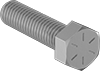
\includegraphics[width=0.7\textwidth]{imgs/hhcs.png}
			\caption{Hex Head}
		\end{subfigure}\begin{subfigure}[b]{.24\linewidth}
			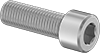
\includegraphics[width=0.7\textwidth]{imgs/shcs.png}
			\caption{Socket Head}
		\end{subfigure}\begin{subfigure}[b]{.24\linewidth}
			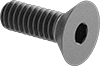
\includegraphics[width=0.7\textwidth]{imgs/fhcs.png}
			\caption{Flathead}
		\end{subfigure}\begin{subfigure}[b]{.24\linewidth}
			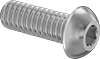
\includegraphics[width=0.7\textwidth]{imgs/bhcs.png}
			\caption{Button Head}
		\end{subfigure}
		
		\begin{subfigure}[b]{.24\linewidth}
			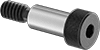
\includegraphics[width=0.7\textwidth]{imgs/shoulderscrew.png}
			\caption{Shoulder Screw}
		\end{subfigure}\begin{subfigure}[b]{.24\linewidth}
			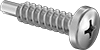
\includegraphics[width=0.7\textwidth]{imgs/stscrew.png}
			\caption{Self-Tapping Screw}
		\end{subfigure}\begin{subfigure}[b]{.24\linewidth}
			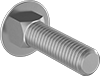
\includegraphics[width=0.7\textwidth]{imgs/carriagebolt.png}
			\caption{Carriage Bolt}
		\end{subfigure}\begin{subfigure}[b]{.24\linewidth}
			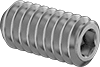
\includegraphics[width=0.7\textwidth]{imgs/grubscrew.png}
			\caption{Grub/Set Screw}
		\end{subfigure}
		\caption{Screw Types}
	\end{figure}
	
	\begin{enumerate}[label=\alph*]
		\item Hex head bolts are good when only side-access is possible, or a cheap solution is needed.
		\item Socket head bolts are preferred. They can be installed in deep wells and have a compact head profile.
		\item Flat head screws need to be installed into holes that have been countersunk to the same angle as the head of the screw. They allow for a flush, smooth installation. However, they have a smaller hex than socket heads of the same thread diameter. This makes them more prone to stripping the head out.
		\item Button head screws provide a smooth surface without the need to countersink the surface. They still have a smaller-diameter hex than socket-heads, though, so are generally unpreferred.
		\item Shoulder screws are special-use screws. The shoulder (unthreaded) portion is precision ground and usually a larger diameter than the thread. This allos them to be used as pins or pivot points.
		\item Self-tapping screws have specially formed tips based on what material they are designed to tap into. They thread into material directly; a tap is not required to form threads, and in plastic and wood, are generally stronger.
		\item Carriage bolts have a rounded head without any means of being driven externally. Instead, the square portion sitting under the thread mates with the material it bolts together (either a plate with the corresponding female portion, or a soft material like wood conforms to the square). Plow bolts are the same principle, but are flat-headed.
		\item Set Screws (often called grub screws) are used to lock down on another piece of material. Commonly seen to secure hubs to shafts. They have very small hexes relative to their thread diameter and are notorious for stripping out.
	\end{enumerate}
	
	There are a lot of different head types that can be put on these bolts as well. 
	
	\begin{figure}[H]
		\centering
		\begin{subfigure}[b]{.15\linewidth}
			
\includegraphics[width=0.7\textwidth]{imgs/head_ext_hex.png}
			\caption{External Hex}
		\end{subfigure}\begin{subfigure}[b]{.15\linewidth}
			
\includegraphics[width=0.7\textwidth]{imgs/head_hex.png}
			\caption{Socket Hex}
		\end{subfigure}\begin{subfigure}[b]{.15\linewidth}
			
\includegraphics[width=0.7\textwidth]{imgs/head_slot.png}
			\caption{Flathead}
		\end{subfigure}\begin{subfigure}[b]{.15\linewidth}
			
\includegraphics[width=0.7\textwidth]{imgs/head_phil.png}
			\caption{Phillips}
		\end{subfigure}\begin{subfigure}[b]{.15\linewidth}
			
\includegraphics[width=0.7\textwidth]{imgs/head_torx.png}
			\caption{Torx}
		\end{subfigure}\begin{subfigure}[b]{.15\linewidth}
			
\includegraphics[width=0.7\textwidth]{imgs/head_robertson.png}
			\caption{Robertson}
		\end{subfigure}
		\caption{Drive Heads}
	\end{figure}
	
	\begin{enumerate}[label=\alph*]
		\item External Hex - very robust, prefferred only when side access is available
		\item Socket Hex - Preferred head, very easy to access from head-on or in a deep pocket
		\item Flathead - Not preferred; very easy to have driver fall out
		\item Phillips - Not preferred; very easy to cam out. When driving a phillips screw, apply inward pressure, and make sure the proper size driver is selected (it should fit nicely).
		\item Torx - Preferred, but more expensive and tools are less common. Very difficult to strip out.
		\item Robertson - Somewhat preferred, but not common. Usually found only in wood screws.
	\end{enumerate}
	
	Preload is very important in threaded joints. For shear loads as illustrated in Figure \ref{fig:bolted_joint}, the load is best carried by the friction inbetween plates rather than shearing the pin itself, since the load is distributed across a larger area.
	
	\begin{figure}[H] \label{fig:bolted_joint} \centering
		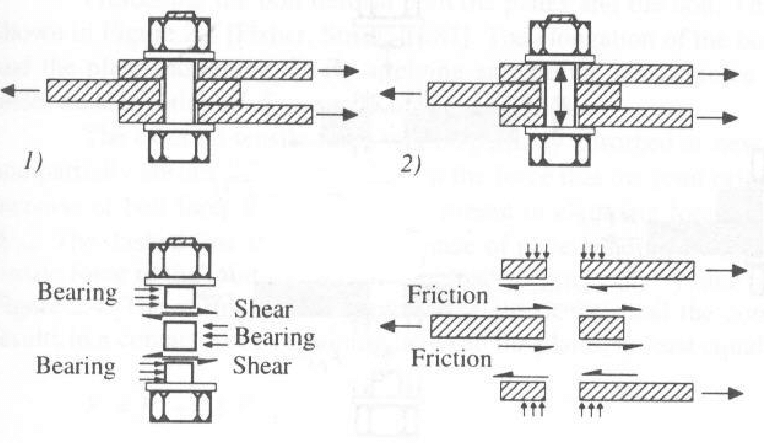
\includegraphics[width=0.5\textwidth]{imgs/bolt_preload.png}
		\caption{Aspects of a Bolted Joint}
	\end{figure}
	
	Spreading the load across the greater area increases rigidity and decreases backlash, egg-out, and strength. However, too much torque can dig the head of the bolt/screw into the underlying material, especially if it is soft (like plastic, or even aluminum), so a washer may be needed to further distribute the load.
	
	\begin{figure}[H]
		\centering
		\begin{subfigure}[b]{.24\linewidth}
			\includegraphics[width=0.7\textwidth]{imgs/plainwasher.png}
			\caption{Plain Washer}
		\end{subfigure}\begin{subfigure}[b]{.24\linewidth}
			\includegraphics[width=0.7\textwidth]{imgs/machinewasher.png}
			\caption{Machine Washer}
		\end{subfigure}\begin{subfigure}[b]{.24\linewidth}
			\includegraphics[width=0.7\textwidth]{imgs/fenderwasher.png}
			\caption{Fender Washer}
		\end{subfigure}
		\caption{Plain Washers of Differring Sizes}
	\end{figure}
	
	Bolts thread into nuts, which can be replaced if they strip out. But if the material a screw threads into strips, then that whole piece will need to be replaced or repaired- which can be even more costly. There are some considerations that can be made to ensure success when using integral threads. The first is to make sure to use coarse (not fine) threads in soft materials like aluminum or plastic. Another option is to use thread inserts.
	
	\begin{figure}[H]
		\centering
		\begin{subfigure}[b]{.24\linewidth}
			\includegraphics[width=0.5\textwidth]{imgs/helicoil.png}
			\caption{Helicoil}
		\end{subfigure}\begin{subfigure}[b]{.24\linewidth}
			\includegraphics[width=0.5\textwidth]{imgs/tanglock.png}
			\caption{Tang-Lock Insert}
		\end{subfigure}\begin{subfigure}[b]{.24\linewidth}
			\includegraphics[width=0.5\textwidth]{imgs/rivnut.png}
			\caption{Rivnut}
		\end{subfigure}\begin{subfigure}[b]{.24\linewidth}
			\includegraphics[width=0.5\textwidth]{imgs/pemnut.png}
			\caption{PEM Nut}
		\end{subfigure}
		
		\begin{subfigure}[b]{.24\linewidth}
			\includegraphics[width=0.5\textwidth]{imgs/heatset.png}
			\caption{Heat-Set Insert}
		\end{subfigure}\begin{subfigure}[b]{.24\linewidth}
			\includegraphics[width=0.5\textwidth]{imgs/teenut.png}
			\caption{Tee Nut}
		\end{subfigure}\begin{subfigure}[b]{.24\linewidth}
			\includegraphics[width=0.5\textwidth]{imgs/woodsti.png}
			\caption{Wood Tapping Insert}
		\end{subfigure}
		\caption{Thread Inserts}
	\end{figure}
	
	\begin{enumerate}[label=\alph*]
		\item Helicoils can be installed after a thread strips out, or before it does preventatively. They are a coiled piece of metal formed like threads.
		\item Tang-lock inserts work much like helicoils, but are solid-bodied rather than coiled, and have locking tangs that can be hammered down on installation to make sure the insert doesn't back out.
		\item Rivnuts (Rivet Nuts) can be installed into holes in thin metal to provide ample threads for fastening. They work much like rivets (more on those later), but need a special tool.
		\item PEM nuts serve the same purpose as rivnuts, but are simply pressed into the sheet they are to be installed in.
		\item Heat-Set Inserts are for plastic. They are instaled by heating them up with a soldering iron and pressing them into thermoplastic. An excellent addition to 3D prints.
		\item Tee Nuts are meant to be pressed into wood, much like a PEM nut.
		\item Wood tapping inserts are much like tang-lock inserts, but with larger wings suitable for wood.
	\end{enumerate}
	
	Threaded joints have one big weakness, and that is their subsceptibility to vibration. There are many solutions to try and combat this.
	
	\begin{figure}[H]
		\centering
		\begin{subfigure}[b]{.24\linewidth}
			\includegraphics[width=0.8\textwidth]{imgs/lockwire.png}
			\caption{Safety/Lock Wire}
		\end{subfigure}\begin{subfigure}[b]{.24\linewidth}
			\includegraphics[width=0.8\textwidth]{imgs/threadlocker.jpeg}
			\caption{Threadlocker}
		\end{subfigure}\begin{subfigure}[b]{.24\linewidth}
			\includegraphics[width=0.5\textwidth]{imgs/nylock.png}
			\caption{Nylock Nut}
		\end{subfigure}\begin{subfigure}[b]{.24\linewidth}
			\includegraphics[width=0.7\textwidth]{imgs/kaynut.png}
			\caption{Kay/Jet Nut}
		\end{subfigure}
		
		\begin{subfigure}[b]{.24\linewidth}
			\includegraphics[width=0.5\textwidth]{imgs/jamnut.png}
			\caption{Jam Nut}
		\end{subfigure}\begin{subfigure}[b]{.24\linewidth}
			\includegraphics[width=0.5\textwidth]{imgs/nordlock.png}
			\caption{Nordlock Washer}
		\end{subfigure}\begin{subfigure}[b]{.24\linewidth}
			\includegraphics[width=0.5\textwidth]{imgs/splitlock.png}
			\caption{Split Lock Washer}
		\end{subfigure}\begin{subfigure}[b]{.24\linewidth}
			\includegraphics[width=0.5\textwidth]{imgs/castlenut.png}
			\caption{Castle Nut}
		\end{subfigure}
		\caption{ Thread Locking Strategies}
	\end{figure}
	
	\begin{enumerate}[label=\alph*]
		\item Lock wire requires tedious installation and bolts with cross-drilled holes to feed the stainless steel wire through. That said, when it is installed properly, it is virtually impossible to fail, and as such is the standard in many aerospace applications. 
		\item Threadlocker (sometimes referred to by the brand name Loctite) comes in various different strengths and can be used on metal-on-metal contact. It's basically long-cure, specially formulated superglue. However, it does attack many plastics, so be careful! It also requires time to cure to full strength, so is not an instant fix, but must be premeditated.
		\item Nylock nuts have a nylon patch that deforms when the threads pass through it. The nut should be installed metal-side first, nylon-side last. These are limited use (<50 uses).
		\item Kay/Jet nuts (metal locknuts) work on the same idea as nylock nuts, but in this case, the nut is deformed and interferes with the thread. It is quite difficult to thread into these nuts. These are extremely limited use (<5 uses) but will work in extreme temperatures, unlike nylocks.
		\item Jam Nuts are simply a second nut jammed up against the first nut. This enables easy adjustment, but is not a very positive way of locking something in place.
		\item Nordlock washers are special ratcheting washers which prevent loosening when properly torqued. There are many different types of locking washers.
		\item Split lock washers are cheap washers which arguably do not actually prevent loosening.
		\item Castle nuts are nuts with slots through which a pin can be fed, locking the nut to the bolt it is secured to. A very robust method.
	\end{enumerate}
	
	\subsection{Rivets}
	
	Pop rivets are a light and cheap method of fastening. However, they require a special gun and are one-time use. They must be drilled out in order to remove them. They are weaker than bolts, so more must be used, but overall, they are a lighter option. Installation is also more picky than bolting. However, they can still be a time-saver over bolts (when disassembly is not a factor).
	
	Rivets are specified by diameter and 'grip length'; the amount of material sandwiched together they can grip. Rivets should be installed to close-fit holes, straight, and with the plates already pulled together.
	
	\begin{figure}[H] \centering
		\includegraphics[width=0.39\textwidth]{imgs/rivet_proc.jpeg}
		\includegraphics[width=0.6\textwidth]{imgs/rivet_install.jpeg}
		\caption{Left: Process of Rivet Installation. Right: Diagnosing rivet failures.}
	\end{figure}
	
	
	\subsection{Shaft Retention}
	
	Retaining rings are used to constrain objects along a shaft.
	
	\begin{figure}[H]
		\centering
		\includegraphics[width=0.45\textwidth]{imgs/shaft_snapringgroove.png}
		\includegraphics[width=0.45\textwidth]{imgs/snapringtool.jpeg}
		\caption{Left: Shaft with groove for retaining ring. Right: Snap ring pliers.}
	\end{figure}
	
	\begin{figure}[H]
		\centering
		\begin{subfigure}[b]{.24\linewidth}
			\includegraphics[width=0.8\textwidth]{imgs/eclip.png}
			\caption{E-Clip}
		\end{subfigure}\begin{subfigure}[b]{.24\linewidth}
			\includegraphics[width=0.8\textwidth]{imgs/int_snapring.png}
			\caption{Internal Snap Ring}
		\end{subfigure}\begin{subfigure}[b]{.24\linewidth}
			\includegraphics[width=0.5\textwidth]{imgs/ext_snapring.png}
			\caption{External Snap Ring}
		\end{subfigure}\begin{subfigure}[b]{.24\linewidth}
			\includegraphics[width=0.7\textwidth]{imgs/pushonring.png}
			\caption{Push-On Ring}
		\end{subfigure}
		
		\begin{subfigure}[b]{.24\linewidth}
			\includegraphics[width=0.7\textwidth]{imgs/spiralring.png}
			\caption{Spiral Ring}
		\end{subfigure}\begin{subfigure}[b]{.24\linewidth}
			\includegraphics[width=0.7\textwidth]{imgs/circlip.png}
			\caption{Circlip}
		\end{subfigure}\begin{subfigure}[b]{.24\linewidth}
			\includegraphics[width=0.7\textwidth]{imgs/shaftcollar.png}
			\caption{Shaft Collar}
		\end{subfigure}
		\caption{Shaft Retaining Technologies}
	\end{figure}
	
	
	\begin{enumerate}[label=\alph*]
		\item E-clips can be pushed into a groove. They are aided by the use of a snap-ring tool to splay them apart, but it is not necessary. They can be installed without passing the clip over the end of a shaft.
		\item Internal snap rings are compressed by a snap-ring tool, and installed into the groove of a housing.
		\item External snap rings are expanded by a snap-ring tool, and installed over the groove of a shaft.
		\item Push-on rings are pushed onto shafts (no groove needed) and (ideally) ratchet on, never coming off.
		\item Spiral rings are wound into grooves. They're annoying and rare.
		\item Circlips are very stiff, low-profile retaining clips.
		\item Shaft collars are heavy, high-profile, but easily removable and adjustable. They come in different bore shapes (hex, round, keyed). They come in two-piece and one-piece varieties.
	\end{enumerate}
	
	\subsection{Adhesives}
	
	Adhesives are useful from time to time.
	
	\begin{enumerate}[label=\alph*]
		\item Retaining compound (e.g. Loctite Green) is meant to bond bearings to their housings, and is very good at it.
		\item Epoxies are two-part adhesives that are mixed immediately prior to application. They can cure quickly.
		\item Cryanacrolate (superglue) adhesives are good for many plastics. Loctite has a good design/test guide for different plastic/glue combinations.
		\item Tapes can be quite useful. Good duct tape and gaffers tape can be used for high-fidelity prototyping and quick fixes.
		\item Pressure-sensitive tape (e.g. 3M VHB) can be incredibly strong. Follow manufacturer's directions.
		\item Velcro and dual-lock can produce easy-but-secure removable components.
	\end{enumerate}

\chapter{Motors}
 {\slshape \scshape ``Move That Gear Up!"}
 \\
 
 Motors are one of the fundamental aspects of mechatronic systems - they're where power is transformed from electrical into mechanical. There are many, many different types of motors, and some of these (like servomotors) are actually complex systems built on top of motors.

\section{Brushed and Brushless Motors}

To begin with, let's talk about the most essential types of motors: Brushed DC motors.

\begin{figure}[H]\centering
\includegraphics[width=0.6\textwidth]{img_Mechatronics_Motors_brushed.png}
\caption{Brushed Motor Anatomy}
% todo: better image
\end{figure}

"Brushed" DC motors have two electrical leads on them - power in, and power out. Current is directed first through carbon 'brushes'. These brushes rub against a "commutator", forming a rotary switch. This switch determines which coil(s) on the rotor fire, and which direction they fire in. When a coil turns on, it pushes/pulls against the permanent magnets, which creates a torque, thus turning the rotor. When the rotor turns, the commutator redirects power into a new set of coils. This process repeats, syncing the firing of the coils with the position of the rotor, in order to produce torque. 

% commutator image

This setup is very cheap, as it does not require any complex electronics. However, such motors are not particularly robust, as these brushes can be a source of friction and wear.

Can we eliminate these problematic brushes? Brushless DC motors, as per the name implies, do exactly that.

In brushless motors, the rotor contains the permanent magnets, and the electromagnets are fixed in place.
\begin{figure}[H]\centering
\includegraphics[width=0.6\textwidth]{img_Mechatronics_Motors_brushless.png}
\caption{Brushless Motor Anatomy}
% todo: better image
\end{figure}

An Electronic Speed Controller (ESC) creates three AC waveforms. These waveforms are fed into the motor. The motor can be either a 'delta' or 'wye' configuration (it doesn't change the fundamental behavior). This alternating current creates alternating forces, which rotate the rotor.

The hard electrical connections are more robust, but does add some cost and complexity as the ESC is required in order for this motor to work. However, there is one major issue with this setup: what happens when the AC waveform is no longer in sync with the rotation of the rotor? Well, a loss of torque occurs. These motors are not very well-equipped to handle high torques, and so are better equipped for high-RPM, low-load applications, such as propellers on hobby aircraft.

However, we could employ an encoder to read the rotor's position, and feed that information back into the ESC. If the ESC can be programmed to read this signal, it can keep the waveform in sync with the rotor's movement, creating higher torque.

Brushless motors have a few other subtle advantages.

Since the waveform is electronically controlled, it can be finer tuned to achieve peak performance (mechanical power output or efficiency). The elimination of brushes also eliminates one source of friction, so their efficiency is generally higher.

The coils of brushed motors, being fixed to the rotor, have very little surface area by which to dissipate heat- the heat has to disspiate out primarially through the shaft. Brushless motors' coils are fixed to the case, which has a much higher surface area, and so they can reject heat better, keeping the motor cool and efficient.

% Summary table?

\section{Empirical Motor Behavior}

Like many complex systems, analysis is good for designing the system, but for using it, gathering empirical test data is a much more practical approach. It turns out that the test data (almost) always follows a general shape, with different numbers. This shape is often called a 'motor curve'. Motor manufacturers typically provide some of these specs in some form. \href{http://motors.vex.com}{\color{red}motors.vex.com} is a very good site as well for FRC, as they conduct third-party testing using the same procedure on each motor, so the results are an apples-to-apples comparison.

% Example datasheet

The first portion of the motor model we'll look at is torque, varying with operating speed, while all parameters are held constant (generally, at the maximum rated voltage). The data typically looks like so:

\begin{figure}[H] \centering \label{fig:motor_torque_curve}
\begin{tikzpicture}[x=4.0in,y=1.2in]
  %\fill[lightgray] (1.0,0)--(0,1.0)--(0,0)--cycle;
  \draw[black] (-0.1,0)--(1.2,0) node[pos=0.5,below]{Speed $\omega$, RPM};
  \draw[black] (0,-0.1)--(0,1.2) node[pos=0.5,above,rotate=90,teal]{Torque $T$, N-m};

  \draw[teal, ultra thick] (1.0,0)--(0,1.0);
\end{tikzpicture}
\caption{General Motor Torque Curve}
\end{figure}

This could be expressed as an equation for a line,
\begin{align} \label{eq:motor_torque_curve}
  T = T_{max} \frac{\omega-\omega_{max}}{\omega_{max}}
\end{align}

With the torque and velocity data, we can compute the power; the rate at which torque is done, or

\begin{align} \label{eq:shaft_power}
  P = T \cdot \omega
\end{align}

Substituting Equation \ref{eq:motor_torque_curve} into \ref{eq:shaft_power} yields the following equation for the power curve.

\begin{align} \label{eq:motor_power_curve}
  P = T_{max} \frac{(\omega_{max}-\omega) \omega}{\omega_{max}}
\end{align}

Note: $\omega$ must be in rad/s, not RPM.

\begin{figure}[H] \centering \label{fig:motor_torque_curve}
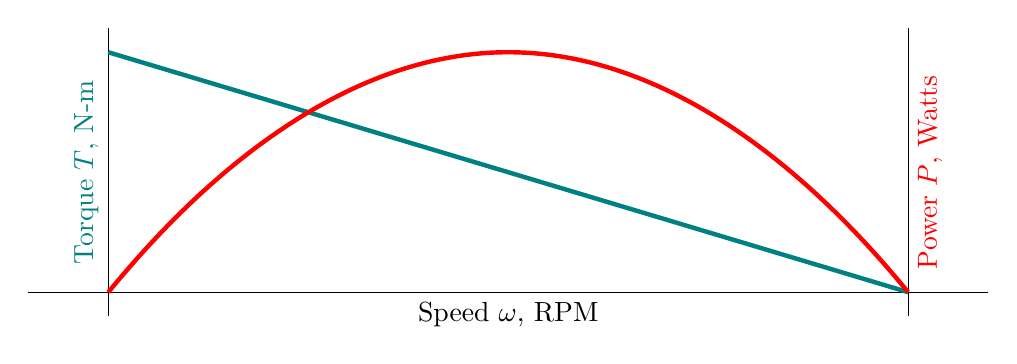
\begin{tikzpicture}[x=4.0in,y=1.2in]
  %\fill[lightgray] (1.0,0)--(0,1.0)--(0,0)--cycle;
  \draw[black] (-0.1,0)--(1.1,0) node[pos=0.5,below]{Speed $\omega$, RPM};
  \draw[black] (0,-0.1)--(0,1.1) node[pos=0.5,above,rotate=90,teal]{Torque $T$, N-m};
  \draw[black] (1,-0.1)--(1,1.1) node[pos=0.5,below,rotate=90,red]{Power $P$, Watts};

  \draw[teal, ultra thick] (1.0,0)--(0,1.0);
  \draw[red, ultra thick] (0,0) parabola bend (0.5,1.0) (1.0,0.0) ;
\end{tikzpicture}
\caption{General Motor Power and Torque Curve}
\end{figure}

Current ($I$) is how much electricity is drawn. It varies proportionally to torque, so

\begin{align} \label{eq:motor_current_curve}
  I = C T \nonumber \\
  I = C T_{max} \frac{\omega_{max}-\omega}{\omega_{max}}
\end{align}

\begin{figure}[H] \centering
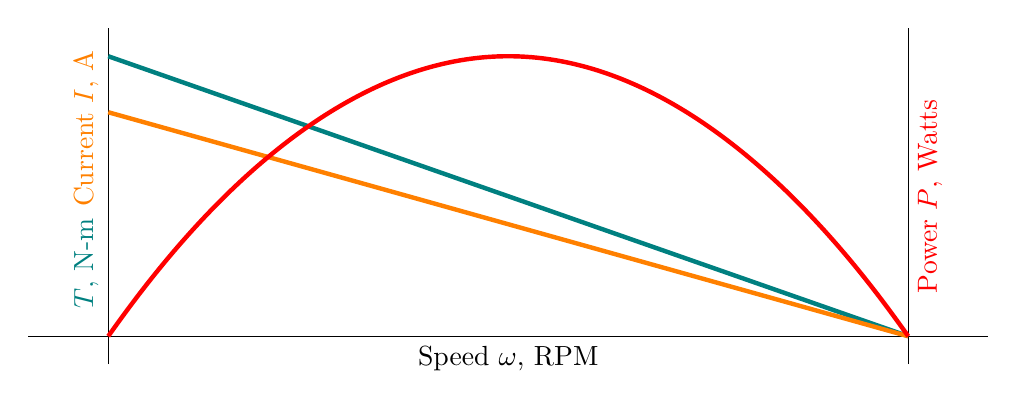
\begin{tikzpicture}[x=4.0in,y=1.4in]
  %\fill[lightgray] (1.0,0)--(0,1.0)--(0,0)--cycle;
  \draw[black] (-0.1,0)--(1.1,0) node[pos=0.5,below]{Speed $\omega$, RPM};
  \draw[black] (0,-0.1)--(0,1.1) node[pos=0.3,above,rotate=90,teal]{$T$, N-m} node[pos=0.7,above,rotate=90,orange]{Current $I$, A};
  \draw[black] (1,-0.1)--(1,1.1) node[pos=0.5,below,rotate=90,red]{Power $P$, Watts};

  \draw[teal, ultra thick] (1.0,0)--(0,1.0);
  \draw[orange, ultra thick] (1.0,0)--(0,0.8);
  \draw[red, ultra thick] (0,0) parabola bend (0.5,1.0) (1.0,0.0) ;
\end{tikzpicture}
\caption{General Motor Current Curve}
\end{figure}

Efficiency ($\eta$) is a ratio of how much mechanical energy is produced per electrical energy spent.

\begin{equation} \label{eq:motor_efficiency_curve}
  \eta = \frac{P_{mech}}{P_{elec}} = \frac{T-M_{friction} \omega}{V I}
  = \frac{[T_{max} \ \frac{(\omega_{max}-\omega)}{\omega_{max}} - M_f] \omega}{V\ C\ T_{max} \frac{(\omega_{max}-\omega)}{\omega_{max}}} \nonumber
\end{equation}

Indeed an ugly equation, let's just plot it with some semi-realistic values.

\begin{figure}[H] \centering
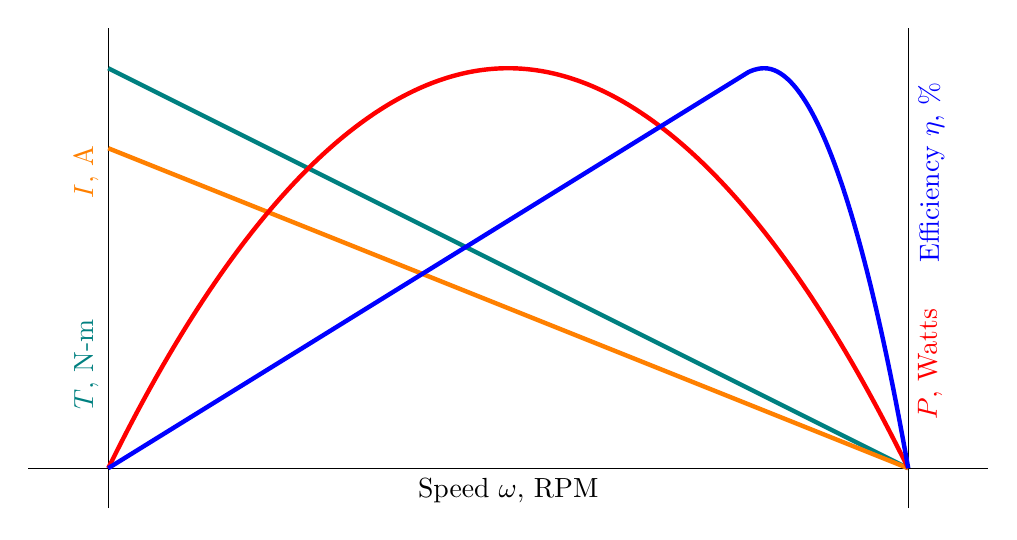
\begin{tikzpicture}[x=4.0in,y=2.0in]
  %\fill[lightgray] (1.0,0)--(0,1.0)--(0,0)--cycle;
  \draw[black] (-0.1,0)--(1.1,0) node[pos=0.5,below]{Speed $\omega$, RPM};
  \draw[black] (0,-0.1)--(0,1.1) node[pos=0.3,above,rotate=90,teal]{$T$, N-m}
  node[pos=0.7,above,rotate=90,orange]{$I$, A};
  \draw[black] (1,-0.1)--(1,1.1) node[pos=0.3,below,rotate=90,red]{$P$, Watts}
  node[pos=0.7,below,rotate=90,blue]{Efficiency $\eta$, \%};

  \draw[teal, ultra thick] (1.0,0)--(0,1.0);
  \draw[orange, ultra thick] (1.0,0)--(0,0.8);
  \draw[red, ultra thick] (0,0) parabola bend (0.5,1.0) (1.0,0.0) ;
  \draw[blue, ultra thick] (0,0)--(0.8,0.99) parabola bend (0.82,1.0) (1.0,0.0) ;
\end{tikzpicture}
\caption{Complete Motor Curve}
\end{figure}

There is a lot going on in this graph! Let's look at some key takeaways:
\begin{itemize}
	\item Motors produce less and less torque as they spin up.
	\item No power is produced when the motor is at maximum speed or maximum torque.
	\item Maximum power is produced at 50\% of maximum speed, which is also at 50\% of maximum torque.
	\item Maximum efficiency occurs somewhere between 75\% and 90\% of free speed.
\end{itemize}

\chapter{Gears, gears, and more gears}
 {\slshape \scshape ``Power is worthless, if improperly wielded"}
 \\

If we have a motor with a pinion of $N_m$ teeth, mating with a driven gear of $N_d$ teeth, we would achieve a gear ratio of

\begin{equation}
  G = \frac{N_d}{N_m} = \frac{\omega_m}{\omega_d} = \frac{T_d}{T_m}
\end{equation}

This also works with belts or sprockets and chain (though you may need to keep an eye on the direction of rotation, as gears can reverse the direction of rotation).

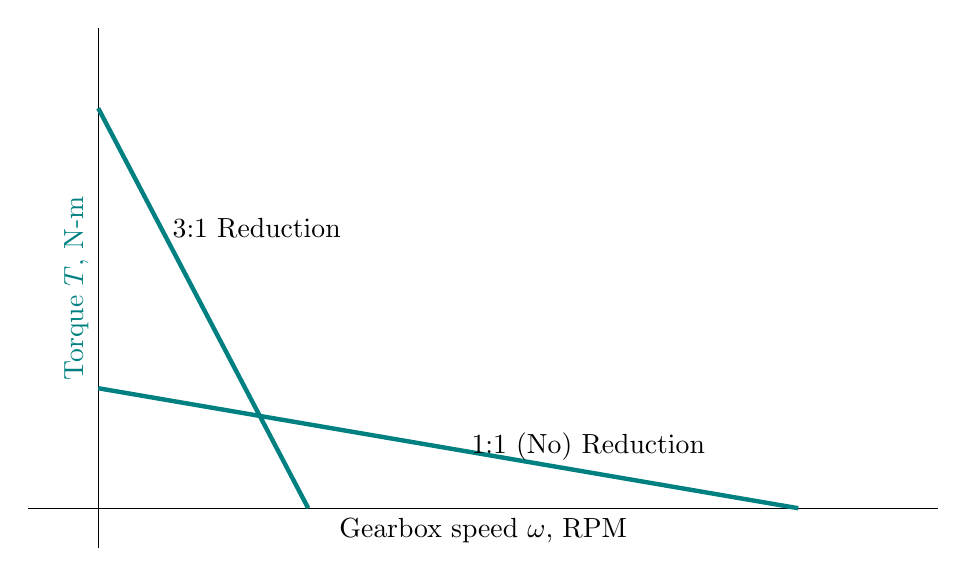
\begin{tikzpicture}[x=3.5in,y=2.0in]
  %\fill[lightgray] (1.0,0)--(0,1.0)--(0,0)--cycle;
  \draw[black] (-0.1,0)--(1.2,0) node[pos=0.5,below]{Gearbox speed $\omega$, RPM};
  \draw[black] (0,-0.1)--(0,1.2) node[pos=0.5,above,rotate=90,teal]{Torque $T$, N-m};

  \draw[teal, ultra thick] (1.0,0)--(0,0.3) node[pos=0.3, above, black]{1:1 (No) Reduction};
  \draw[teal, ultra thick] (0.3,0)--(0,1.0) node[pos=0.7, right, black]{3:1 Reduction};
\end{tikzpicture}


The 3:1 ratio reduces maximum speed, but increases the maximum torque.
It also changes the RPM at which maximum power and efficiency occur.


\end{document}